\documentclass{beamer}
\usepackage[utf8]{inputenc}

\usetheme{Madrid}
\usecolortheme{default}
\usepackage{amsmath,amssymb,amsfonts,amsthm}
\usepackage{txfonts}
\usepackage{tkz-euclide}
\usepackage{listings}
\usepackage{adjustbox}
\usepackage{array}
\usepackage{tabularx}
\usepackage{gvv}
\usepackage{lmodern}
\usepackage{circuitikz}
\usepackage{tikz}
\usepackage{graphicx}

\setbeamertemplate{page number in head/foot}[totalframenumber]

\usepackage{tcolorbox}
\tcbuselibrary{minted,breakable,xparse,skins}



\definecolor{bg}{gray}{0.95}
\DeclareTCBListing{mintedbox}{O{}m!O{}}{%
  breakable=true,
  listing engine=minted,
  listing only,
  minted language=#2,
  minted style=default,
  minted options={%
    linenos,
    gobble=0,
    breaklines=true,
    breakafter=,,
    fontsize=\small,
    numbersep=8pt,
    #1},
  boxsep=0pt,
  left skip=0pt,
  right skip=0pt,
  left=25pt,
  right=0pt,
  top=3pt,
  bottom=3pt,
  arc=5pt,
  leftrule=0pt,
  rightrule=0pt,
  bottomrule=2pt,
  toprule=2pt,
  colback=bg,
  colframe=orange!70,
  enhanced,
  overlay={%
    \begin{tcbclipinterior}
    \fill[orange!20!white] (frame.south west) rectangle ([xshift=20pt]frame.north west);
    \end{tcbclipinterior}},
  #3,
}
\lstset{
    language=C,
    basicstyle=\ttfamily\small,
    keywordstyle=\color{blue},
    stringstyle=\color{orange},
    commentstyle=\color{green!60!black},
    numbers=left,
    numberstyle=\tiny\color{gray},
    breaklines=true,
    showstringspaces=false,
}
\begin{document}

\title 
{2.5.28}
\date{August ,2025}


\author 
{Namaswi -EE25BTECH11060}






\frame{\titlepage}
\begin{frame}{Question}
 Find the projection of the vector 
\[
\vec{a} = 2\vec{i} + 3\vec{j} + 2\vec{k}
\]
on the vector 
\[
\vec{b} = 2\vec{i} + 2\vec{j} + \vec{k}.
\]
\end{frame}



\begin{frame}{Given data}
\begin{table}[h!]
\centering
\begin{tabular}{|c|c|c|c|}
\hline
\textbf{Vector} & \textbf{i-component} & \textbf{j-component} & \textbf{k-component} \\
\hline
$\vec{a}$ & 2 & 3 & 2 \\
\hline
$\vec{b}$ & 2 & 2 & 1 \\
\hline
\end{tabular}
\caption{Components of vectors $\vec{a}$ and $\vec{b}$}
\end{table}

 
\end{frame}

\begin{frame}{Formulae}
 Projection of vector $\vec{A}$  on $\vec{B}$ is given by \\
\begin{align}
\frac{\vec{A}^\top\vec{B}}{||\vec{B}^2||}\vec{B}\\
\frac{\begin{pmatrix} 2 & 3 & 2 \end{pmatrix}\begin{pmatrix}
    2 \\ 2 \\ 1 \end{pmatrix}}{2^2+2^2+1^2}\vec{B}\\
\end{align}
\end{frame}


\begin{frame}{Theoretical Solution}
\begin{align*}
=\frac{2^2+(3)(2)+(2)(1)}{2^2+2^2+1^2}\begin{pmatrix} 2 \\ 2 \\1 \end{pmatrix}\\
=\frac{12}{9}\begin{pmatrix} 2 \\ 2 \\1 \end{pmatrix}\\
=\frac{4}{3}\begin{pmatrix} 2 \\ 2 \\1 \end{pmatrix}
=\begin{pmatrix}
    \frac{8}{3} \\ \frac{8}{3}  \\    \frac{4}{3}
    \end{pmatrix}\\
    The \;projection\; vector \;is \;given\; by \frac{{8}}{3}\,\mathbf{i} + \frac{8}{3}\,\mathbf{j}+ 
\frac{4}{3}\,\mathbf{k}
\end{align*}
\end{frame}


 


 

\begin{frame}[fragile]
    \frametitle{C Code }

    \begin{lstlisting}

 #include <stdio.h>

int main() {
    double a[3] = {2, 3, 2};
    double b[3] = {2, 2, 1};
    double dot = 0.0, normB2 = 0.0;
    for(int i = 0; i < 3; i++) {
        dot += a[i] * b[i];
        normB2 += b[i] * b[i]; }
    double factor = dot / normB2;
    double proj[3];
    for(int i = 0; i < 3; i++) {
        proj[i] = factor * b[i];}
    printf("Projection of a on b = (%.2lf)i + (%.2lf)j + (%.2lf)k\n",
           proj[0], proj[1], proj[2]);
 return 0;
}
 \end{lstlisting}
\end{frame}

\begin{frame}[fragile]
    \frametitle{Python Code}
    \begin{lstlisting}
 import numpy as np
import matplotlib.pyplot as plt
from mpl_toolkits.mplot3d import Axes3D

# Define vectors
a = np.array([2, 3, 2])
b = np.array([2, 2, 1])

    \end{lstlisting}
\end{frame}

\begin{frame}[fragile]
    \frametitle{Python Code}
    \begin{lstlisting}
 # Compute projection of a onto b
proj_scalar = np.dot(a, b) / np.dot(b, b)
proj = proj_scalar * b

# Plotting
fig = plt.figure()
ax = fig.add_subplot(111, projection='3d')

# Plot origin
origin = [0, 0, 0]


    \end{lstlisting}
\end{frame}

\begin{frame}[fragile]
    \frametitle{Python Code}
    \begin{lstlisting}
 

# Plot vectors
ax.quiver(*origin, *a, color='blue', label='Vector a', linewidth=2)
ax.quiver(*origin, *b, color='green', label='Vector b', linewidth=2)
ax.quiver(*origin, *proj, color='red', label='Projection of a on b', linestyle='dashed', linewidth=2)

# Labels and settings
ax.set_xlim([0, 4])
ax.set_ylim([0, 4])
ax.set_zlim([0, 4])
ax.set_xlabel('X')
ax.set_ylabel('Y')
ax.set_zlabel('Z')
ax.set_title('Projection of Vector a onto Vector b')
ax.legend()
plt.tight_layout()
plt.show()

    \end{lstlisting}
\end{frame}

\begin{frame}[fragile]
    \frametitle{Python Code}
    \begin{lstlisting}
 import ctypes

# Load the shared C library
lib = ctypes.CDLL("./libprojection.so")   # use "projection.dll" on Windows

# Define argument and return types
lib.projection.argtypes = [ctypes.POINTER(ctypes.c_double),
                           ctypes.POINTER(ctypes.c_double),
                           ctypes.POINTER(ctypes.c_double)]
lib.projection.restype = None

    \end{lstlisting}
\end{frame}
\begin{frame}[fragile]
    \frametitle{Python Code}
    \begin{lstlisting}
 lib.projection.restype = None

# Define vectors a and b
a = (ctypes.c_double * 3)(2, 3, 2)
b = (ctypes.c_double * 3)(2, 2, 1)
proj = (ctypes.c_double * 3)()

# Call C function
lib.projection(a, b, proj)

# Print result
print(f"Projection of a on b = ({proj[0]:.2f})i + ({proj[1]:.2f})j + ({proj[2]:.2f})k")

    \end{lstlisting}
\end{frame}
 


\begin{frame}{Plot}
    \centering
    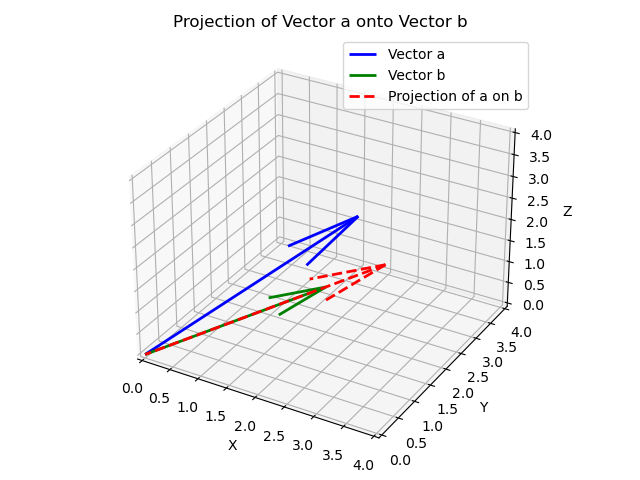
\includegraphics[width=\columnwidth, height=0.8\textheight, keepaspectratio]{Figure_3.png}     
\end{frame}


\end{document}